\fancyhead{}
\fancyfoot{}


\lhead{Realizar un radio enlace y t�nel redundante}

\subsection{Configuraci�n Estaci�n.}
La configuraci�n de nuestra estaci�n es mucho m�s sencilla ya que como estaci�n tendremos que configurar �nicamente los siguientes par�metros:\\

\textbf{General}\\
\textbf{Name:} Permite cambiar el nombre de la interface en la que os encontramos.\\\
\textbf{Type:} Muestra el tipo de chip que utiliza la mini PcI.MTU (unidad m�xima de transferencia): Expresa el tama�o en byte de la unidad de datos m�s grande que puede enviarse usando un Protocolo de Internet. \\
\textbf{Wireless}\\
\textbf{Mode:} Designa el modo de funcionamiento de la interfaz en este caso AP Bridge.\\
\textbf{Band:} hace referencia al rango de frecuencia sobre el cual se va a trabajar. 
\textbf{Frecuencia:} Especifica el canal permanente sobre el cual se va a traficar informaci�n dado por el AP al que se conecta.\\
\textbf{SSID:} Ya que la estaci�n pertenecer� a la misma red del AP, esta tendr� que utilizar el mismo SSID.\\
\textbf{Security Profile:} Al igual que con el SSID, la estaci�n debe tener la misma seguridad para comunicar los dos equipos.\\
\textbf{Antena Mode:} Ya que las targejas miniPCI dispones para dos conectores, en el momento que este se conecta en el principal (main), colocamos como antena a, si por el contrario decidimos conectar al otro puerto (aux), el modo ser� antena b.\\
\textbf{Antena Gain:} Ganancia de la antena externa que estemos utilizando (en dBi).\\
\textbf{Tx-Power:} En la opci�n de potencia podremos controlar la potencia de salida de las miniPCI, (en dBi).\\
Escoger el men� \textbf{New Terminal} $\rightarrow$  \textbf{system reset-configuration} 
\begin{figure}[H]
\begin{center}
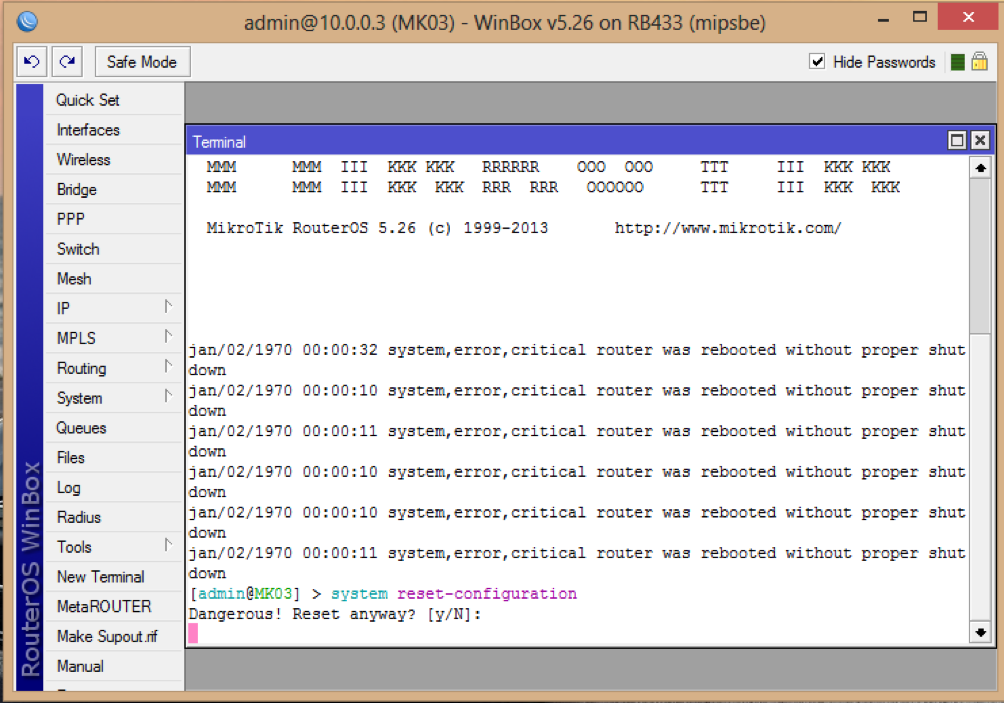
\includegraphics[scale = .5]{./figuras/figura073.png}
\caption{Reestablecer Configuraciones MK3}
\label{reestablecer-configuraciones-mk3}
\end{center}
\end{figure}
 Escoger el men� \textbf{Remove Configuration} 
\begin{figure}[H]
\begin{center}
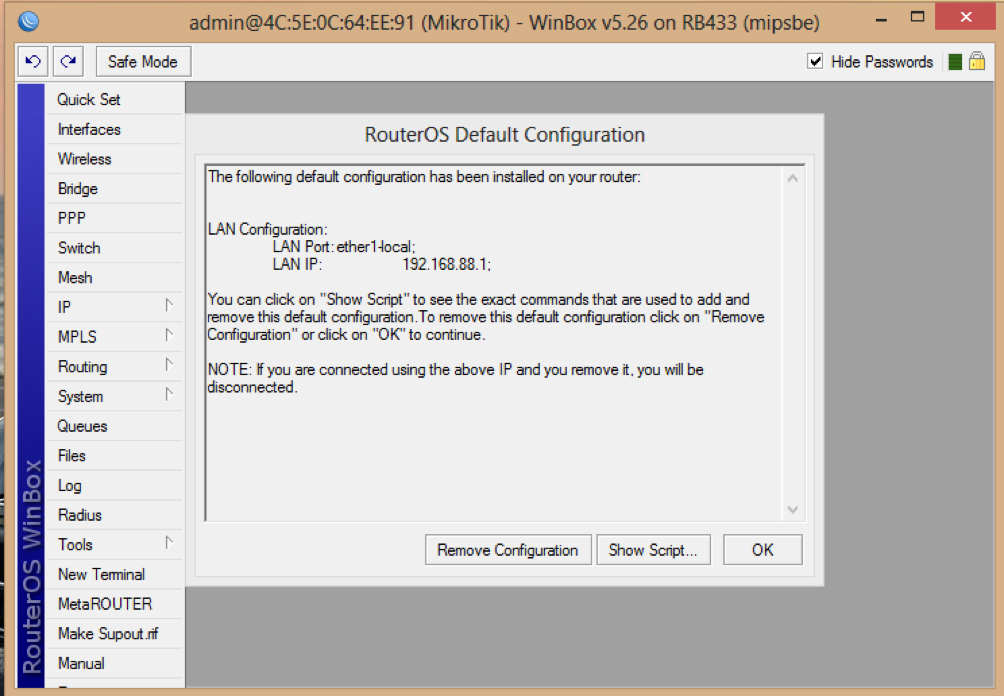
\includegraphics[scale = .5]{./figuras/figura074.png}
\caption{Remover configuraciones}
\label{remover-configuraciones-74}
\end{center}
\end{figure}
 Escoger el men� \textbf{Brige} $\rightarrow$ \textcolor{red}{\textbf{+}}\\
\begin{figure}[H]
\begin{center}
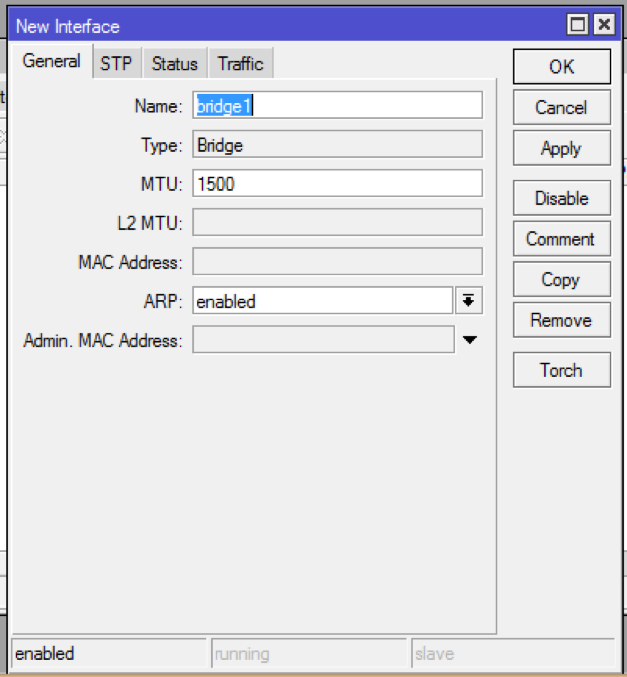
\includegraphics[scale = .5]{./figuras/figura075.png}
\caption{Crear Bridge}
\label{crear-bridge}
\end{center}
\end{figure}
 Escoger el men� \textbf{Bridge} $\rightarrow$  \textbf{Ports} 
\begin{figure}[H]
\begin{center}
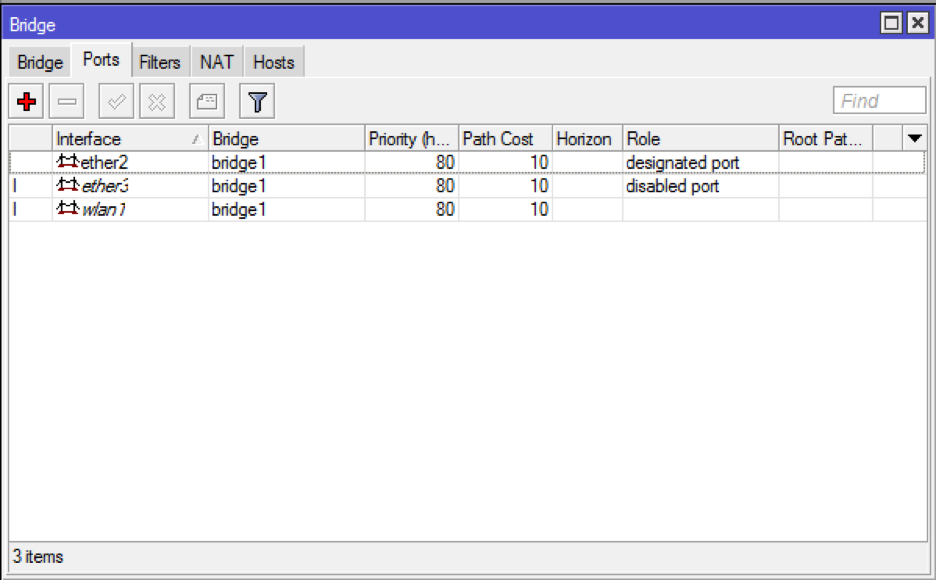
\includegraphics[scale = .5]{./figuras/figura076.png}
\caption{Lista de interfaces en el Bridge}
\label{lista-interfaces-bridge}
\end{center}
\end{figure}
 Escoger el men� \textbf{IP} $\rightarrow$  \textbf{Address}  $\rightarrow$ \textcolor{red}{\textbf{+}}\\
\begin{figure}[H]
\begin{center}
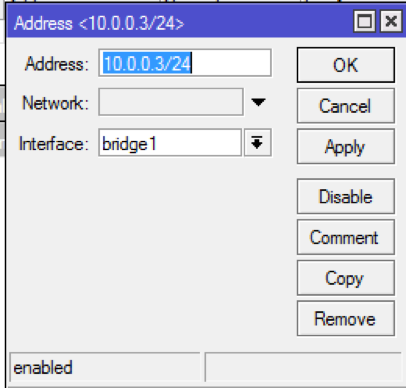
\includegraphics[scale = .5]{./figuras/figura077.png}
\caption{Configurar IP}
\label{configurar-ip}
\end{center}
\end{figure}
 Escoger el men� \textbf{Wireless} 
\begin{figure}[H]
\begin{center}
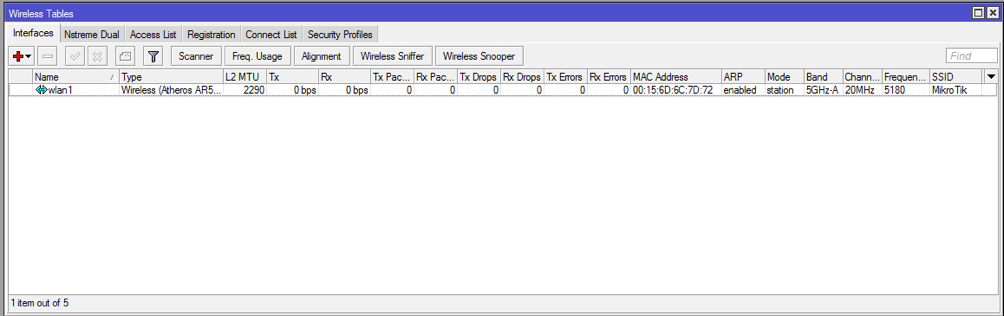
\includegraphics[scale = .5]{./figuras/figura078.png}
\caption{Lista Interfaces Wireless disponibles}
\label{lista-interfaces-wireless-disponibles}
\end{center}
\end{figure}
 Escoger el men� \textbf{Wireless} $\rightarrow$  \textbf{wlan1}  $\rightarrow$ \textbf{Wireless}\\
\begin{figure}[H]
\begin{center}
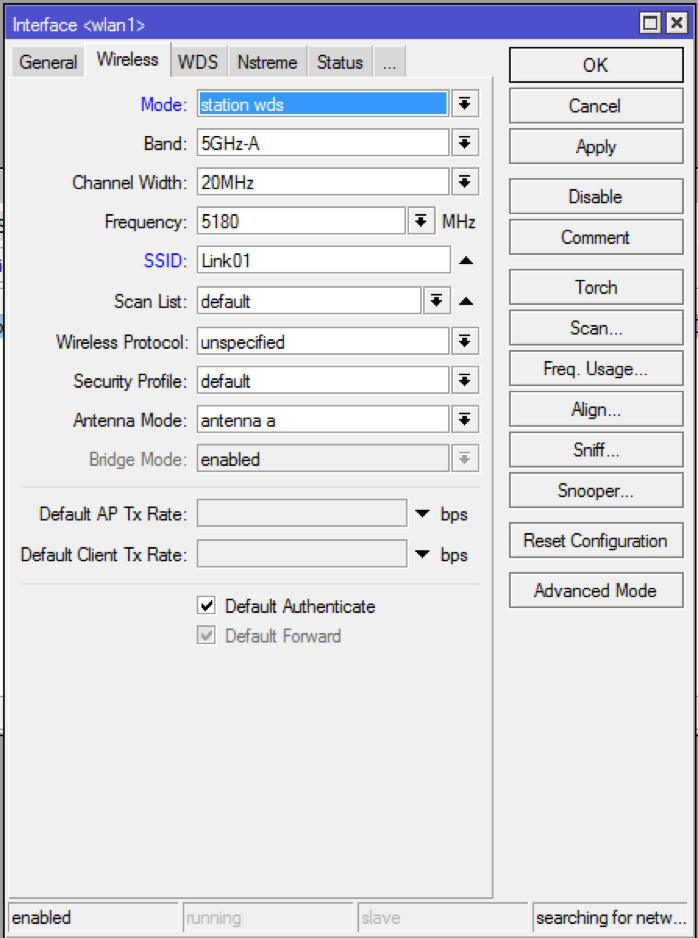
\includegraphics[scale = .5]{./figuras/figura079.png}
\caption{Configurar Wireless Station}
\label{configurar-wireless-station}
\end{center}
\end{figure}
% Bridge y WDS escribir algo sobre estos dos bichos.. 
Escoger el men� \textbf{Wireless} $\rightarrow$  \textbf{wlan1}  $\rightarrow$ \textbf{WDS}\\
\begin{figure}[H]
\begin{center}
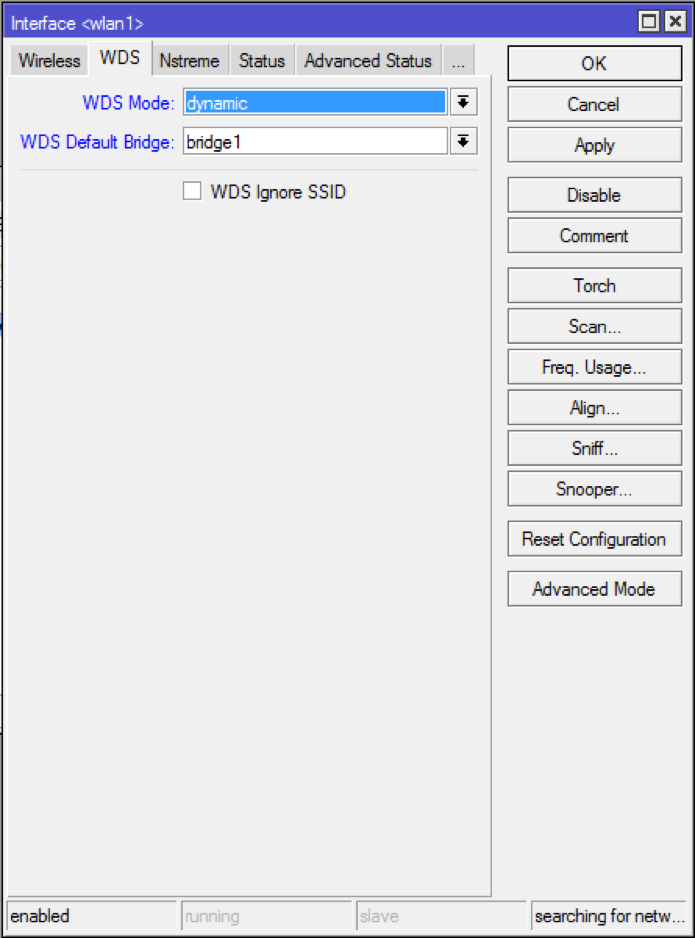
\includegraphics[scale = .5]{./figuras/figura080.png}
\caption{Configura interface en la Bridge y WDS}
\label{configura-interface-bridge-wds}
\end{center}
\end{figure}
 

\newglossaryentry{ietf}
{
name=IETF,
description={The Internet Engineering Task Force (IETF�)}
}
\newglossaryentry{tcp/ip}
{
name=TCP/IP,
description={Protocolo de control de transmisi�n/Protocolo de Internet}
}
